\documentclass[en,11pt]{classes/aghdpl}  % praca w języku angielskim

% Lista wszystkich języków stanowiących języki pozycji bibliograficznych użytych w pracy.
% (Zgodnie z zasadami tworzenia bibliografii każda pozycja powinna zostać utworzona zgodnie z zasadami języka, w którym dana publikacja została napisana.)
\usepackage[english]{babel}

\usepackage[utf8]{inputenc}

% dodatkowe pakiety
\usepackage[dvipsnames]{xcolor}
\usepackage{listings}

\usepackage{mathtools}
\usepackage{amsfonts}
\usepackage{amsmath}
\usepackage{amsthm}
\usepackage{hyperref}
\usepackage[chapter,outputdir=build]{minted}


% --- < bibliografia > ---

\usepackage[
style=numeric,
sorting=none,
%
% Zastosuj styl wpisu bibliograficznego właściwy językowi publikacji.
language=autobib,
autolang=other,
% Zapisuj datę dostępu do strony WWW w formacie RRRR-MM-DD.
urldate=iso8601,
% Nie dodawaj numerów stron, na których występuje cytowanie.
backref=false,
% Podawaj ISBN.
isbn=true,
% Nie podawaj URL-i, o ile nie jest to konieczne.
url=false,
%
% Ustawienia związane z polskimi normami dla bibliografii.
maxbibnames=3,
% Jeżeli używamy BibTeXa:
backend=bibtex
]{biblatex}

\usepackage{csquotes}
% Ponieważ `csquotes` nie posiada polskiego stylu, można skorzystać z mocno zbliżonego stylu chorwackiego.
\DeclareQuoteAlias{croatian}{english}

\addbibresource{bibliography/bibliography.bib}

% Nie wyświetlaj wybranych pól.
%\AtEveryBibitem{\clearfield{note}}


% ------------------------
% --- < listingi > ---
%--- < json listing > ---
\definecolor{delim}{RGB}{20,105,176}
\definecolor{numb}{RGB}{106, 109, 32}
\definecolor{string}{rgb}{0.64,0.08,0.08}

\lstdefinelanguage{json}{
numbers=left,
numberstyle=\small,
frame=single,
rulecolor=\color{black},
showspaces=false,
showtabs=false,
breaklines=true,
captionpos=b,
postbreak=\raisebox{0ex}[0ex][0ex]{\ensuremath{\color{gray}\hookrightarrow\space}},
breakatwhitespace=true,
basicstyle=\ttfamily\small,
upquote=true,
morestring=[b]",
stringstyle=\color{string},
literate=
*{0}{{{\color{numb}0}}}{1}
{1}{{{\color{numb}1}}}{1}
{2}{{{\color{numb}2}}}{1}
{3}{{{\color{numb}3}}}{1}
{4}{{{\color{numb}4}}}{1}
{5}{{{\color{numb}5}}}{1}
{6}{{{\color{numb}6}}}{1}
{7}{{{\color{numb}7}}}{1}
{8}{{{\color{numb}8}}}{1}
{9}{{{\color{numb}9}}}{1}
{\{}{{{\color{delim}{\{}}}}{1}
{\}}{{{\color{delim}{\}}}}}{1}
{[}{{{\color{delim}{[}}}}{1}
{]}{{{\color{delim}{]}}}}{1},
}

% ---- YAML ----
\newcommand\YAMLcolonstyle{\color{red}\mdseries}
\newcommand\YAMLkeystyle{\color{black}\bfseries}
\newcommand\YAMLvaluestyle{\color{blue}\mdseries}

\makeatletter

% here is a macro expanding to the name of the language
% (handy if you decide to change it further down the road)
\newcommand\language@yaml{yaml}

\expandafter\expandafter\expandafter\lstdefinelanguage
\expandafter{\language@yaml}
{
keywords={true,false,null,n},
keywordstyle=\color{darkgray}\bfseries,
basicstyle=\YAMLkeystyle,                                 % assuming a key comes first
sensitive=false,
comment=[l]{\#},
captionpos=b,
numbers=left,
numberstyle=\small,
frame=single,
rulecolor=\color{black},
showspaces=false,
showtabs=false,
breaklines=true,
morecomment=[s]{/*}{*/},
commentstyle=\color{purple}\ttfamily,
stringstyle=\YAMLvaluestyle\ttfamily,
moredelim=[l][\color{orange}]{\&},
moredelim=[l][\color{magenta}]{*},
moredelim=**[il][\YAMLcolonstyle{:}\YAMLvaluestyle]{:},   % switch to value style at :
morestring=[b]',
morestring=[b]",
literate =    {---}{{\ProcessThreeDashes}}3
{>}{{\textcolor{red}\textgreater}}1
{|}{{\textcolor{red}\textbar}}1
{\ -\ }{{\mdseries\ -\ }}3,
}

% switch to key style at EOL
\lst@AddToHook{EveryLine}{\ifx\lst@language\language@yaml\YAMLkeystyle\fi}
\makeatother

\newcommand\ProcessThreeDashes{\llap{\color{cyan}\mdseries-{-}-}}

% ---- YAML end ----

% Użyj czcionki kroju Courier.
\usepackage{courier}

\usepackage{listings}
\lstloadlanguages{TeX}

\lstset{
	literate={ą}{{\k{a}}}1
           {ć}{{\'c}}1
           {ę}{{\k{e}}}1
           {ó}{{\'o}}1
           {ń}{{\'n}}1
           {ł}{{\l{}}}1
           {ś}{{\'s}}1
           {ź}{{\'z}}1
           {ż}{{\.z}}1
           {Ą}{{\k{A}}}1
           {Ć}{{\'C}}1
           {Ę}{{\k{E}}}1
           {Ó}{{\'O}}1
           {Ń}{{\'N}}1
           {Ł}{{\L{}}}1
           {Ś}{{\'S}}1
           {Ź}{{\'Z}}1
           {Ż}{{\.Z}}1,
	basicstyle=\footnotesize\ttfamily,
}

% ------------------------

\AtBeginDocument{
	\renewcommand{\tablename}{Tab.}
	\renewcommand{\figurename}{Fig.}
}

% ------------------------
% --- < tabele > ---

\usepackage{array}
\usepackage{tabularx}
\usepackage{multirow}
\usepackage{booktabs}
\usepackage{makecell}
\usepackage[flushleft]{threeparttable}

% defines the X column to use m (\parbox[c]) instead of p (`parbox[t]`)
\newcolumntype{C}[1]{>{\hsize=#1\hsize\centering\arraybackslash}X}


%---------------------------------------------------------------------------

\author{Kamil~Kaliś and Piotr~Kuglin}
\shortauthor{K.~Kaliś P.~Kuglin}

% \titlePL{Przygotowanie bardzo długiej i pasjonującej pracy dyplomowej w~systemie~\LaTeX}
% \titleEN{Protection of Web Applications with Behavioral Biometrics}

\titlePL{}
\titleEN{Protection of Web Applications with Behavioral Biometrics}


% \shorttitlePL{Przygotowanie pracy dyplomowej w~systemie \LaTeX} % skrócona wersja tytułu jeśli jest bardzo długi
\shorttitleEN{Protection of Web Applications with Behavioral Biometrics}

% \thesistype{Praca dyplomowa magisterska}
\thesistype{Bachelor's Thesis}

% \supervisor{prof. dr hab. Marcin Szpyrka}
\supervisor{Piotr Chołda, PhD}

% \degreeprogramme{Informatyka}
\degreeprogramme{Electronics and Telecommunications}

\date{2020}

% \department{Katedra Informatyki Stosowanej}
\department{Department of Telecommunications}

% \faculty{Wydział Elektrotechniki, Automatyki,\protect\\[-1mm] Informatyki i Inżynierii Biomedycznej}
\faculty{Faculty of Computer Science, Electronics and Telecommunications}

\acknowledgements{We hereby express our thanks to our supervisor – Piotr Chołda, PhD, who was guiding the process of creation of this thesis. The support in granting the needed resources for the study and feedback provided by Mr. Chołda are invaluable.\\
Special thanks to Krzysztof Rusek, PhD – for consulting the approach for proper machine learning model execution.\\
This research was supported in part by PLGrid Infrastructure.
}


\setlength{\cftsecnumwidth}{10mm}

%---------------------------------------------------------------------------
\renewcommand{\theparagraph}{}
\setcounter{secnumdepth}{4}
\brokenpenalty=10000\relax

\begin{document}

\titlepages

% Ponowne zdefiniowanie stylu `plain`, aby usunąć numer strony z pierwszej strony spisu treści i poszczególnych rozdziałów.
\fancypagestyle{plain}
{
	% Usuń nagłówek i stopkę
	\fancyhf{}
	% Usuń linie.
	\renewcommand{\headrulewidth}{0pt}
	\renewcommand{\footrulewidth}{0pt}
}

\setcounter{tocdepth}{2}
\tableofcontents
\clearpage

\chapter{Implementation}\label{ch:implementation}
To fulfill the assumptions of this work, the authors prepared a system that is able to collect and verify the mouse dynamics data.
The high-level flow of the system is presented in Fig.~\ref{fig:overall_system_structure} and provides the basis for further considerations.
\begin{figure}[!hbt]
    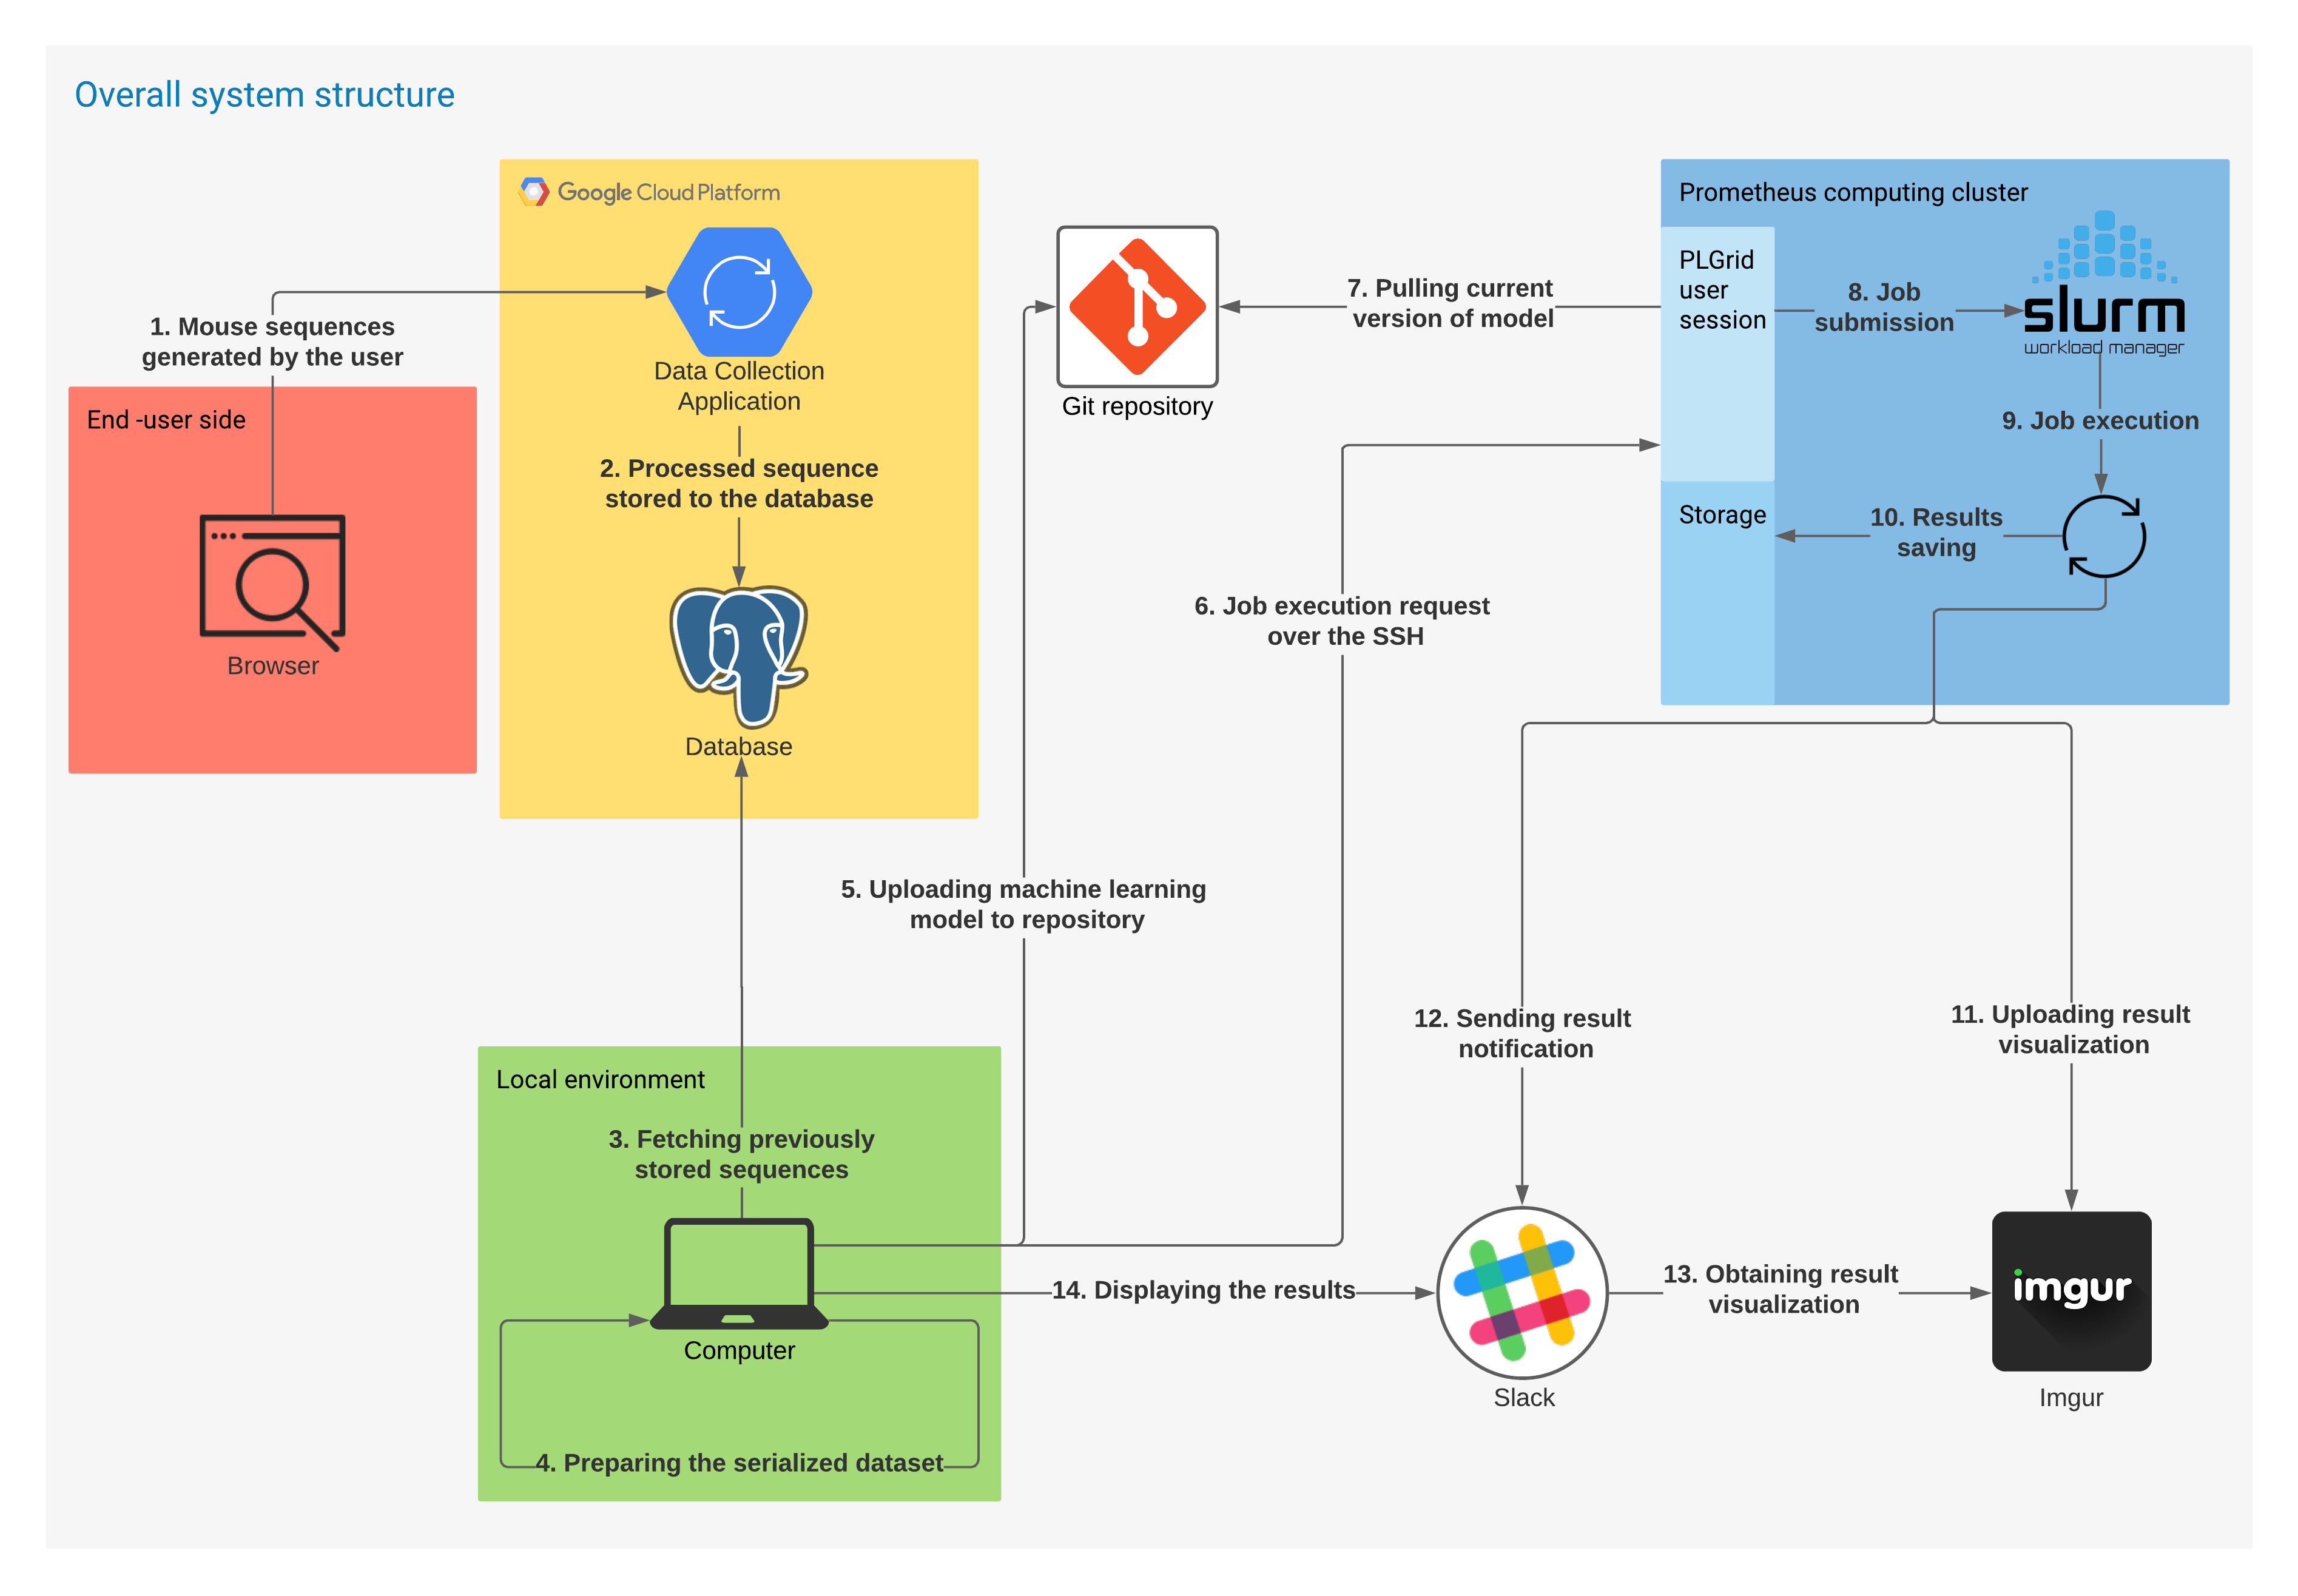
\includegraphics[width=\linewidth]{resources/overall_diagram.png}
    \captionof{figure}{Overall system structure diagram}
    \label{fig:overall_system_structure}
\end{figure}

The entry point for the system is the user's browser that allows the human user as well as a human impersonating bot for access to the prepared website which is hosted on the Internet.
The \mbox{Data Collection}\upperref{itm:data-collection} module which is persisted and operates within a cloud acts as a mouse dynamics data collector, which means that every single mouse event generated by the user on the website is intercepted, transformed and stored in the underlying database (Fig.~\ref{fig:overall_system_structure}, pt. 1 and pt. 2).
The administrator of the presented system is able to retrieve the data from the database in any time (pt. 3).
The downloaded data can be further processed (pt. 4) to the dataset which will be used in machine learning stage.
The administrator of the system should prepare a machine learning model and upload it to the Git repository (pt. 5) which will be then obtained by a computing cluster to perform computation using the model from the observed branch.
Such an approach allows to work on the solution simultaneously by many data scientists and makes it possible to accelerate the research.
The dataset should be uploaded to the computing cluster and persisted in the group's storage that allows using it by many different paralleled computations (not included in the diagram due to decrease of readability).
Each computation is requested from the local computer using prepared Git's `deploy' alias (described in Section~\ref{sec:prometheus-computing-cluster}) that performs a sequence of operations such as establishing the connection to the cluster, fetching the current version of code from the repository and submitting the job to the Slurm\upperref{itm:slurm} workload manager (pt. 6, 7, 8).
The work of the cluster is fully asynchronous because each job is queued and therefore the completion time is unknown.
This is very inconvenient because there is no notification system that allows getting the information about the finished job.
To overcome these limitations, the notification system is proposed as a part of Bot Detection\upperref{itm:bot-detection} module.
The creation of such a system enables the presentation of the results of the computed job in the message as well as the graphs prepared based on the output of the job.
To provide the possibility of sending the images, the notification system uses the external image hosting website called Imgur\upperref{itm:imgur} which allows to upload pictures to the server and host them under the generated \gls{url} (pt. 11).
The results and the graphs are combined into Slack's\upperref{itm:slack} message and then sent to the previously prepared channel by using the webhook \gls{api} (pt. 12, 13).

The further subchapters treat about the implementation details.
At the beginning the Data Collection module is described along with the cloud configuration and performance tests, further, the bot which impersonates the human user and finally the machine learning model alongside the tools such as, among others, a notification module.


\section{Persistence and security}\label{sec:persistence-and-security}
The Data Collection module consists of several submodules, but the core of it is the backend API\footnote{Application Programming Interface} which was written in the 8\textsuperscript{th} version of Java.
The responsibilities of that API are mainly the persistence of captured data and user authentication.
The whole architecture of the API is based on the Spring\footnote{\url{https://spring.io/}} framework which is widely used for such purposes and provides many capabilities in fields of securing and persisting data.
Spring is divided into many projects that create compatible ecosystem and make it possible to develop scalable web applications.
In order to make development in Spring easier and faster the authors of the framework created Spring Boot\footnote{\url{https://spring.io/projects/spring-boot}} which sets up the environment for the developer and provides many easily imported libraries (so-called starters) to use.

To perform database operations using the idea of object–relational mapping (ORM) the implementation of Java Persistence API\footnote{\url{https://www.oracle.com/java/technologies/persistence-jsp.html}} (JPA) provided by Spring Boot was used.
The choice of the database was in the scope of relational databases because the captured data forms the time series which are easily mapped to the structure of the table.
The authors decided to use PostgreSQL because of the popularity and wide range of support.
The data was stored in three different tables.
The first consists of the user's login, password and granted authority which was required to distinguish administrators from ordinary users.
The second one includes sequences of user's captured actions with timestamps, screen resolutions and types of the events.
The last one stores all possible action types with the description.

The collected data is sent to the \gls{api} via Representational State Transfer (REST), which is nowadays one of the most popular interfaces between web applications, because of its simplicity and native support in many different programming languages and technologies.
The schema of the interface was established at the beginning of the work on this module, so it was possible to create the \gls{api} and the fronted application simultaneously.

To protect the data from invalid properties, the input was also validated before saving to the database in such a way that all of persisted data contained all required elements.
Securing such an application from malware users is also important issue, so the access was restricted only for signed users that existed in the database.
The security was provided by using OAuth2\footnote{\url{https://oauth.net/2/}} and JSON Web Token\footnote{\url{https://jwt.io/}} (JWT).
The API was working as a OAuth2 provider which issued JWT tokens and authorized them basing on the user's credentials stored in the database.
Such a mechanism allowed to control access to the application and enforce registration before the use of the system.

The API was prepared with two different switchable profiles: admin oriented and user oriented.
They were created to provide flexibility in accounts creation~---~respectively~---~only by admin and anyone.
In further work only user oriented profile was used.
\section{Presentation and reverse proxy}\label{sec:reverse-proxy}
The second core submodule created for the purpose of collecting the data from the users is the frontend application exposed to the internet.
This can be split further into two different functional modules~--- client and server-side.

\subsection{Client side module}\label{subsec:client-side-module}
The client-side module is an end-user presentation layer that is built with the HTML5 and CSS3~--- technologies that are the core and standard for modern web applications nowadays.
HTML is a widely used markup language used to create hypertext documents and CSS is used as a style-sheet for modifying the design of web documents.
The content of the website is a free, prebuilt template taken from the Colorlib\footnote{\url{https://colorlib.com/}} collection which web templates are licensed under the CC BY 3.0 License\footnote{Creative Commons Attribution 3.0 License --- \url{https://creativecommons.org/licenses/by/3.0/}}.
The mechanism that collects users' mouse actions is designed as a "plugin" script, meaning that the template can be changed easily, so different styled environments that serve various purposes can be used to collect the data.

To use the system and participate in the research, an interested user is required to first accept the consents of usage of the website as well as accept the usage of the cookies and then registration is allowed and required, and afterward, the user is redirected to the login page.
To persists consistency of the registration and login, the custom static web pages were created to be easily transferable between the templates.
On each document, the FAQ panel with more information regarding the project is exposed as a drop-down list.
To authenticate, users are required to provide the credentials to log in to the system.
These credentials are then sent through https --- which means that they are secured and encrypted --- to the reverse proxy server which then performs some action to authenticate a user, sets the cookie with granted JWT token and redirects the user to the homepage.
More on the user authentication and the token obtaining sequence is described in
The whole sequence is described and shown in subsection~\ref{subsec:server-side-module}).

After a successful login, the token allows for site usage and ensures the identity of the user.
From now on, the actions performed by the user are recorded into the batches and sent to the API every two seconds.
The event listeners are awaiting four different action types: mouse move, mouse-down, mouse-up, mouse wheel action.
Collected actions are packed into JSON object and sent to the server side API (described in~\ref{subsec:server-side-module}) --- the fields included are shown in the Listing~\ref{listing:mouse-events-json-schema}.

\begin{listing}[H]
    \inputminted[
    linenos,
    autogobble,
    frame=single,
    framesep=2mm,
    labelposition=bottomline,
    baselinestretch=1.2,
    fontsize=\footnotesize
    ]{json}{resources/mouse-event-json-schema.json}
    \caption{JSON schema for mouse event batches}
    \label{listing:mouse-events-json-schema}
\end{listing}

\subsection{Server side module}\label{subsec:server-side-module}
The server side module is build with Node.js\footnote{\url{https://nodejs.org/}} runtime with the Express\footnote{\url{https://expressjs.com/}} framework on the top of it.
Node.js is an asynchronous JavaScript runtime, which is widely used to build high-end, scalable commercial applications.
Express is light-weight and simple to use, yet powerful web framework for Node.js, which allows for a fast and convenient HTTP server set-up server for serving the static web documents over the internet.
This module is serving the purpose of reverse proxy between clients and the backend API.

The main responsibilities of the reverse proxy are signing up the user, token granting, validation and caching, serving static web documents storing and passing the data to for persistence.
When a new user tries to sign-up, secured with TLS credentials from the sign-up form are sent to one of the proxy endpoints, where they are then passed to the backend API.
Because the backend is not exposed anywhere over the public network, there is no need to secure the credentials with TLS.\\
The user is granted JWT Access and Refresh tokens after logging in using the login form.
The user credentials are secured with TLS and received by proxy API, whereas the proxy server is additionally appending the Client id and Client secret for OAuth2 server to the request "Authorization" header, as the proxy server authenticates to OAuth2 server with HTTP Basic authentication scheme.
Credentials of the user that wishes to log in are included in the body of the request.
When the user is properly authenticated, the OAuth2 server responds with a valid JWT token which is then set as a cookie with HttpOnly, Secure, and SameSite strict options.
When the token is successfully granted, it is also saved to the Redis, which is a simple to use key-value NoSQL database suitable for caching.
The retrieval of such a token is very fast, so this is serving the purpose of the caching system, which results in a great efficiency improvement and lower response time of the server.
For each interaction and request for resources, the user has to hold a valid JWT Token.
First, the token is searched in the cache database.
If it does not figure there, the proxy server is attempting to check the token with the backend OAuth2 server.
If the server responds with Bad Request status or the access token is not set on the user request, the refresh token is being used for access token renewal.
The complete sequence visualization can be seen in \mbox{Fig.~\ref{fig:jwt-sequence}}.
The proxy server is storing the user mouse data received from the client side and periodically passes it to the backend API for persistence.




% Propably should be included elsewhere, maybe appendix?
\begin{figure}[!hbt]
    
    \centering
    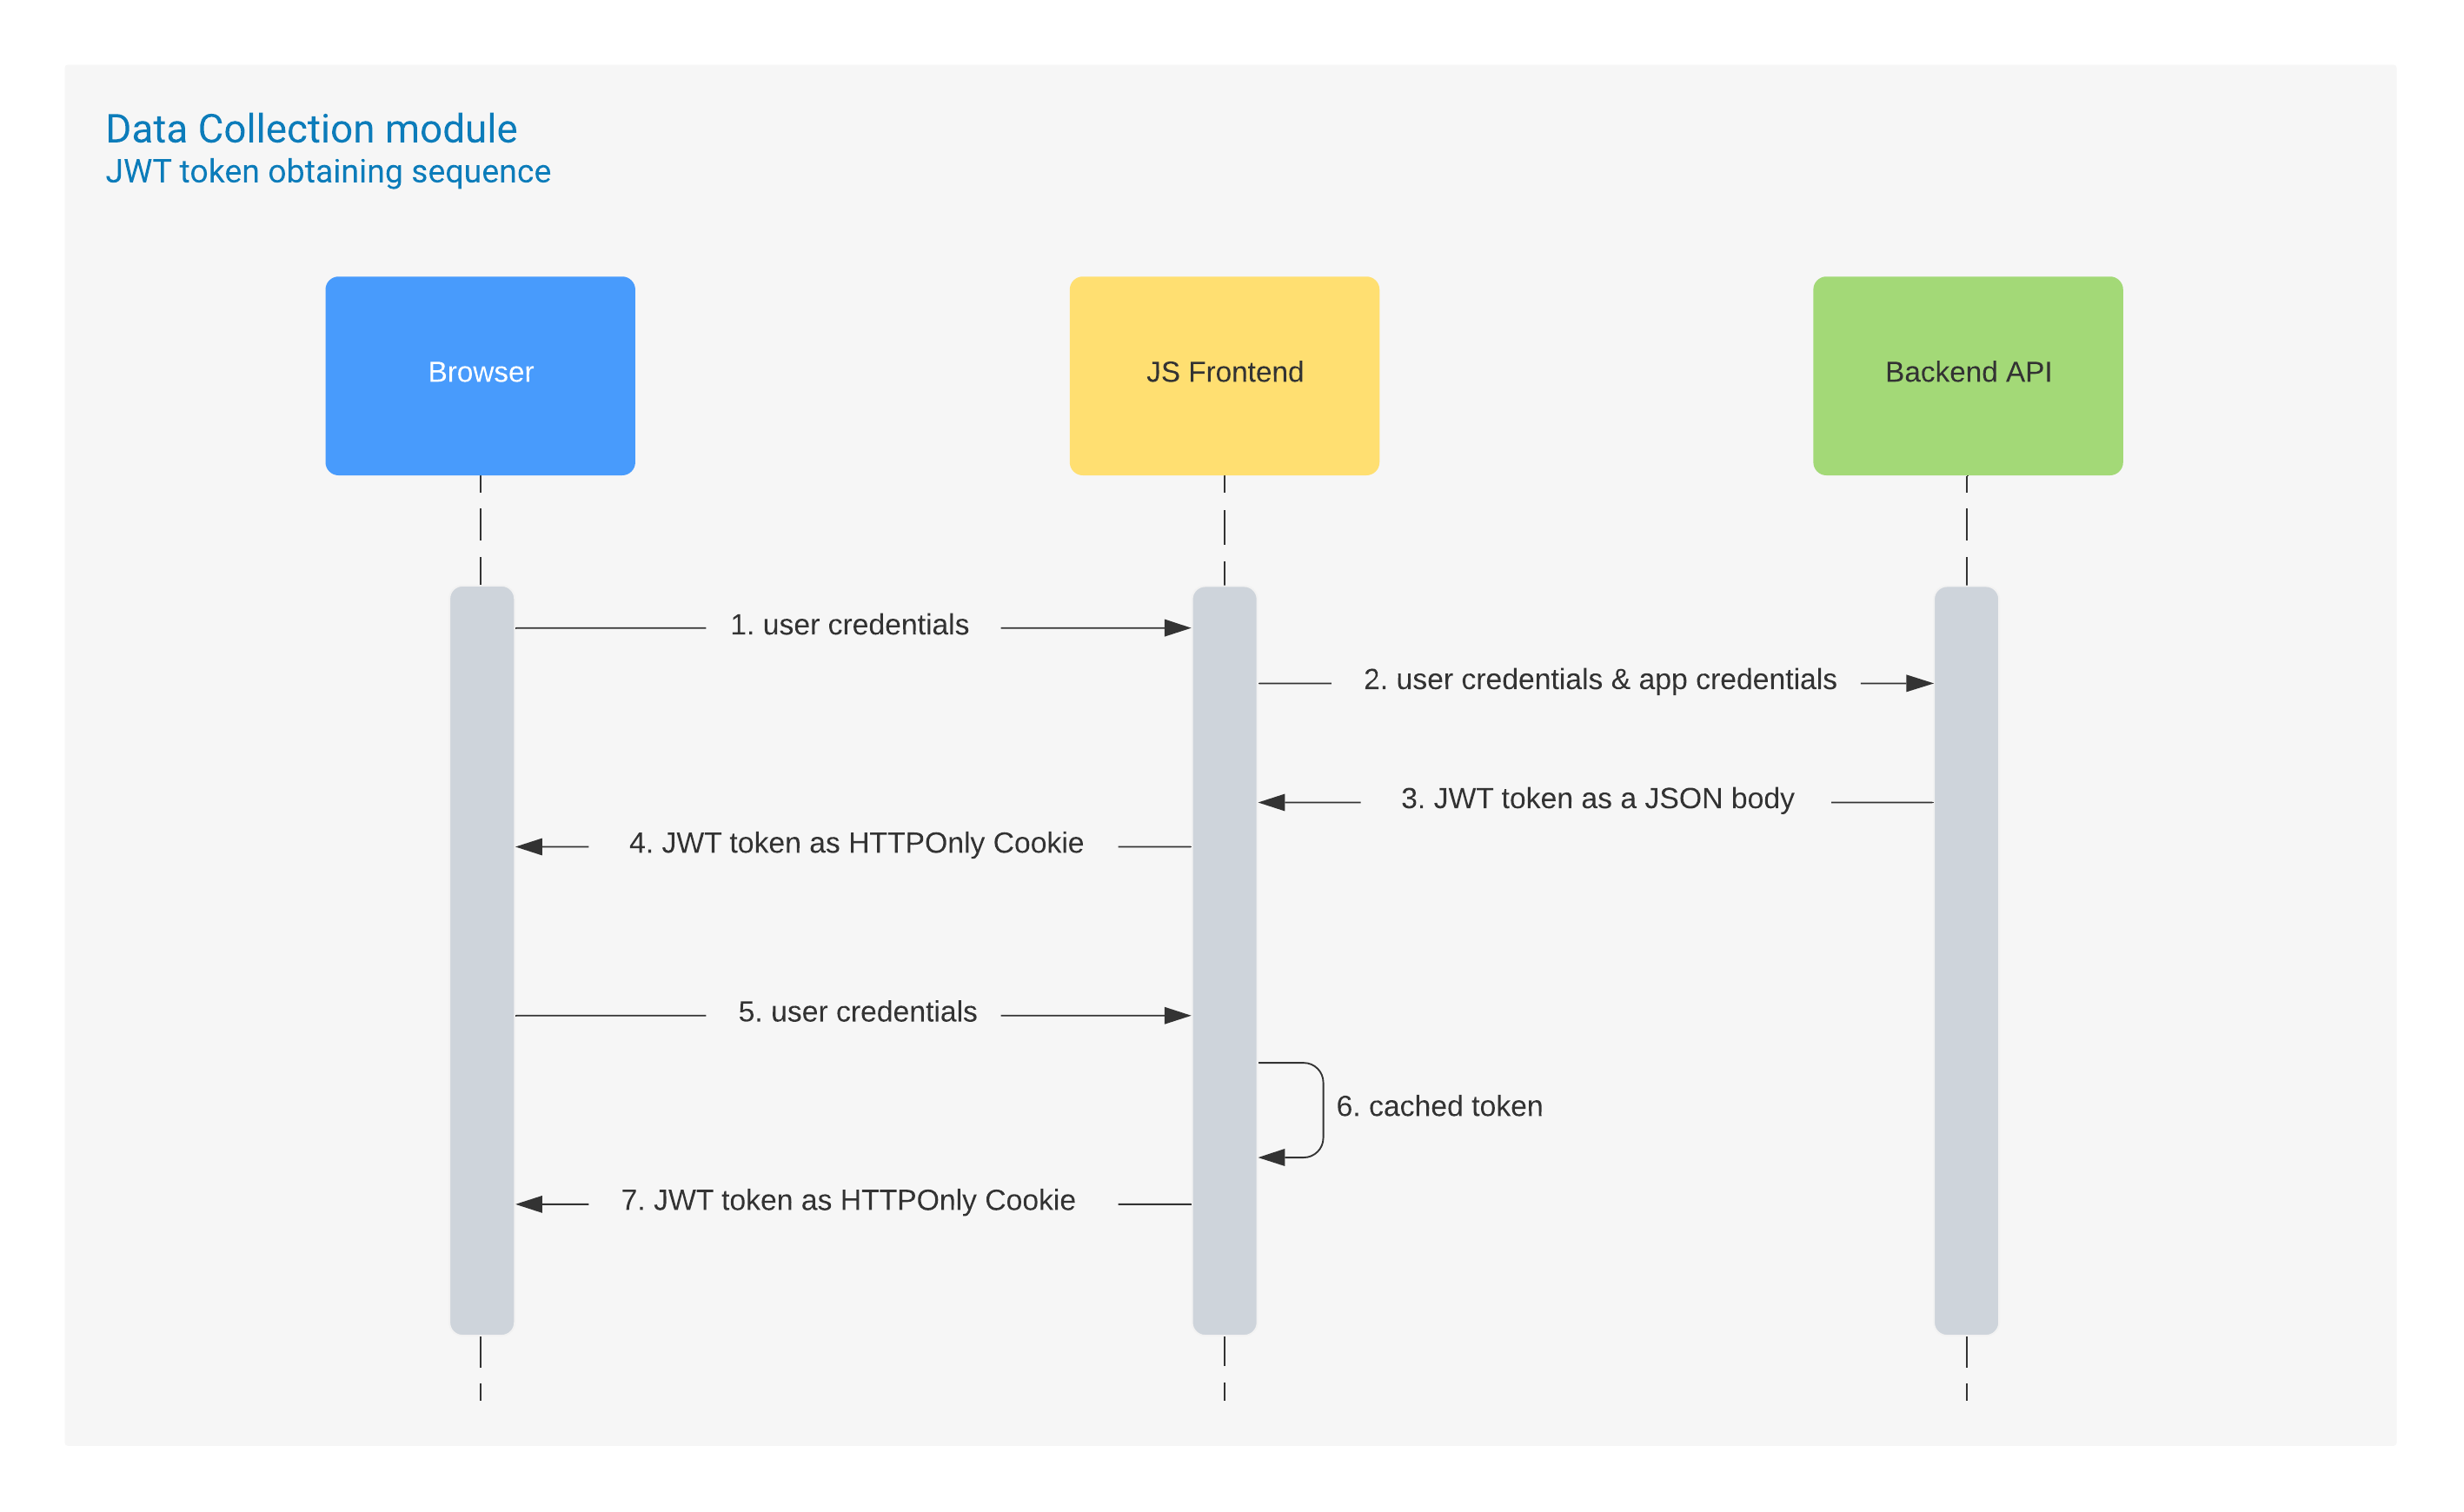
\includegraphics[width=\linewidth]{resources/jwt_sequence_diagram.png}
    \captionsetup{width=\linewidth}
    \captionof{figure}{JWT token obtaining sequence}
    \label{fig:jwt-sequence}
\end{figure}
\section{Performance tests}\label{sec:performance-tests}
The solutions presented in the previous sections were deployed to the Heroku Cloud Application Platform\upperref{itm:heroku} to deliver the possibility of using the system among a wide range of users.
Heroku as a cloud provider has a free pricing plan for non-commercial apps, which is suitable for scientific usage such as this thesis.
The deployment process is performed using the idea of containerization based on Docker\upperref{itm:docker} which is a convenient way of application delivery to the Web server.
To enable such a possibility, the \mbox{Dockerfiles} with container configuration description were prepared for both frontend and backend services and also docker-compose configuration files were created to allow easy testing and development in the local environment.

In order to deliver reliable and efficient product to the users, the performance tests were prepared using JavaScript programming language in the Node.js environment.
Those tests cover mainly the token exchange and refreshment, and also allow to test the behavior of application during increased load produced by using the system by many different users.
The results of the tests showed that the Heroku free pricing plan had some limitations regarding database storage volume and response time from the application.
It turned out that the database in such a plan permit to store only 20,000 rows overall which is unacceptable for the data stream with the time resolution measured in milliseconds because a single user may cause exceeding the limit in just a few minutes, which disqualifies the Heroku as a service provider for a multi-user environment.
Moreover, the described cloud system suspends the work of the application when it is idle.
Waking the application up takes a very long time (up to the minute or more), which is manifested in a usage lag after 30 minutes without any Web traffic.
Described issues with the Heroku Cloud Application Platform forced the authors to find another suitable cloud provider.

\section{Deployment and orchestration}\label{sec:deployment-and-orchestration}
In order to overcome the issues described in the section \ref{sec:performance-tests}, the cloud providers' research was conducted, and based on the results it was decided to adopt the \gls{gcp} (Google Cloud Platform)\upperref{itm:gcp} as a deployment environment.
In the scope of the conducted research, some popular cloud providers were considered, such as \gls{gcp} and \gls{aws} (Amazon Web Services)\upperref{itm:aws}.
Due to the similar costs of both options, the choice was directed by the prior experience that authors had with the \gls{gcp}.

Unlike Heroku, \gls{gcp} had no free pricing plan, but it does not restrict the usage of resources and therefore it met the project assumptions, and moreover, it has some extra advantages like native support for containers orchestration.
The latter is provided by using Kubernetes\upperref{itm:kubernetes}, the open-source solution introducing flexible deployments, scaling and container management.
Those features drastically simplify working with application development in a cloud but require additional setup and configuration files.

Kubernetes natively supports the usage of Docker containers so the ones prepared before can be reused, but the deployment process requires a so-called Deployment configuration files that enable tuning the resources assigned to the single instance of an application and also the number of the replicas of the application.
The basic unit managed by Kubernetes is Pod which may consist of many single Docker containers, but in this work the Pod is associated with a single container of application.
The described scaling method is known as Horizontal Pod Scaling and can be seen in the Fig.~\ref{fig:gcp_diagram} as a several same Pods in single Deployment.
It improves reliability and allows to increase the limit of the maximal load accepted by a single deployment of the application because the load is split into the mirror instances of the same application that work in parallel.

\begin{figure}
    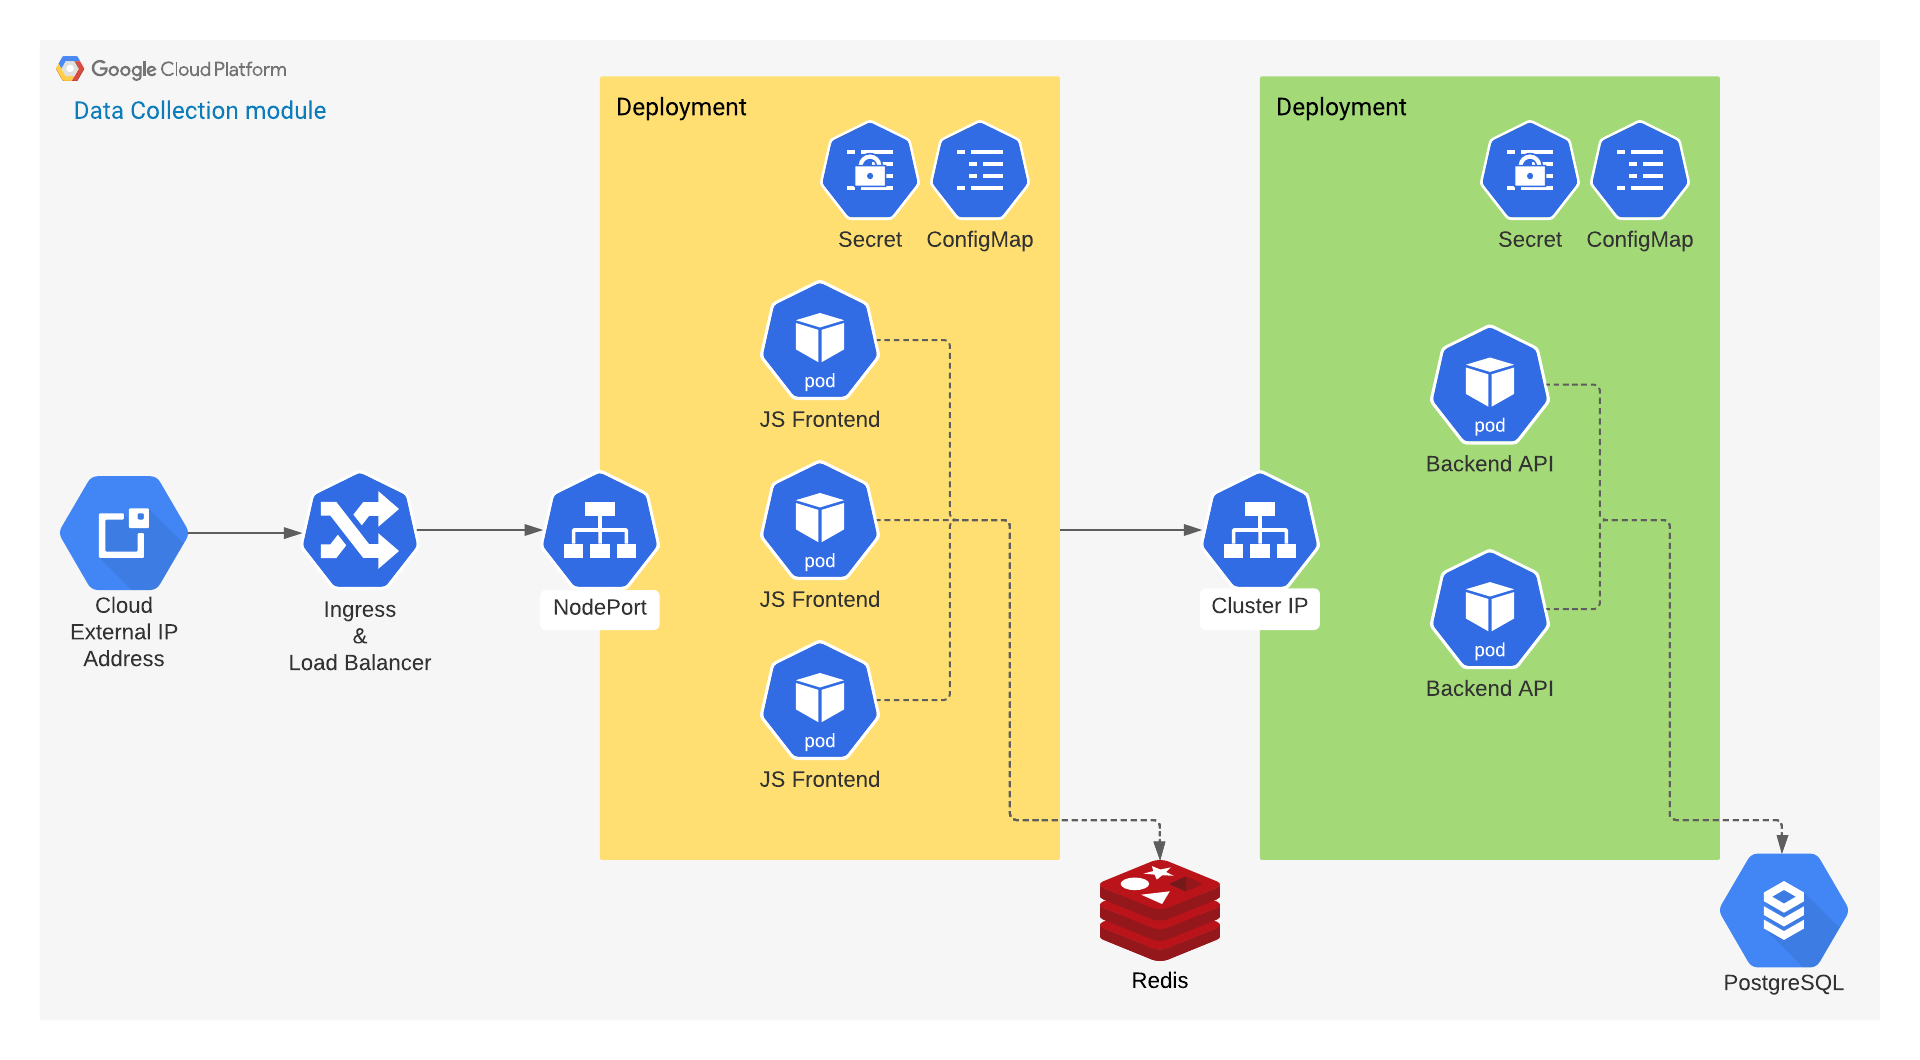
\includegraphics[width=\linewidth]{resources/gcp_diagram}
    \captionof{figure}{Cloud architecture}
    \label{fig:gcp_diagram}
\end{figure}

To deliver the load to all of the mirror applications, Kubernetes uses Services as an entry point to a group of Pods that are managed by one Deployment (in the Fig.~\ref{fig:gcp_diagram} they are drawn on the edge of the Deployment rectangles to mark their gateway nature).
The Service exposes the Deployment under the single \gls{dns} name and updates the underlying IP address in cases of its change, but it also works as a load balancer which distributes the load among the managed Pods.
Kubernetes has several different Service types but in this work two of them are used: Cluster IP that exposes the Deployments in the scope of Kubernetes but hides them from external access and NodePort that permits the access using port-forwarding.
The latter one is dictated by the usage of Google Cloud HTTP(S) load balancer and it also requires additional configuration by using an Ingress and obtaining the static external IP address.

To provide encryption of connection, \gls{tls} should be used, which requires the \gls{ssl} Server Certificate, which can be issued only for existing valid domain names, thus the authors were forced to buy such a domain name, while the certificate is issued by \gls{gcp}.

The configuration also includes some sensitive data, such as database credentials, OAuth2 secret, and SSH-RSA keys, thus the Secrets are used with encoded content.
The insensitive data are included in ConfigMaps that are similar to the Secrets but their content is plain text.
These configurations are matched to the appropriate component by labels and therefore they are drawn inside the Deployment rectangles in Fig.~\ref{fig:gcp_diagram}, in practice they can be mounted as volumes basing on the component labels and can also expose their values as environmental variables.

The whole architecture of the collector system is presented in Fig.~\ref{fig:gcp_diagram}, but the figure has several simplifications such as a way of database deployment.
In contrast to the Redis cache database, the main database instance is not deployed in Kubernetes itself, but the Cloud SQL from \gls{gcp} available services with \mbox{PostgreSQL} is used to achieve straightforward management and reliability.

\section{Custom bot}\label{sec:custom-bot}
In order to prepare a dataset that consists of two classes --- the valid user and human impersonating bot, the custom bot was prepared.

The main idea behind this module is to first create scenarios that next could be executed by the bot software.
To achieve the most convenient creation of scenarios, the authors prepared a utility to record the coordinates and actions of the mouse.
Using this approach, the bot could impersonate a user in a more natural way.
Recorded mouse events are stored as a \gls{yaml} schema, which is a human-readable standard for data serialization.
The structure of a \gls{yaml} scenario schema is shown in Listing~\ref{listing:bot-events-yaml-schema}.

\begin{listing}[ht]
    \inputminted
    [
    linenos,
    autogobble,
    xleftmargin=0.7cm,
    xrightmargin=0.7cm,
%    frame=single,
    framesep=2mm,
    labelposition=bottomline,
    baselinestretch=1.2,
    fontsize=\footnotesize
    ]{yaml}{resources/bot-scenario-schema.yaml}
    \caption{YAML schema for bot event scenarios}
    \label{listing:bot-events-yaml-schema}
\end{listing}

After the scenarios are recorded, the mechanism to execute them is required.
The Custom Bot executor script reads the \gls{yaml} file and loads it to the memory as a list of events, that is then traversed.
The executor script performs an action stored as an "event" filed at the coordinates $(x, y)$.
If the coordinates are different than the current mouse position, the cursor is moved, but to make it more natural, movement is based on the Bézier curve concept.
The Bézier curves are used to effectively represent a smooth curve on a computer screen, as stated by D. F. Rogers~\cite{bezier-curves}.
Knowing this, this concept can be used to simulate smooth human-like movements.

To be able to run a set of scenarios, the module introduces a so-called "batch runner" for predefined cases.
This automation saves a lot of time and effort because a set of scenarios can be executed at once to generate data for the bot class.


\chapter{Implementation}\label{ch:implementation}
To fulfill the assumptions of this work, the authors prepared a system that is able to collect and verify the mouse dynamics data.
The high-level flow of the system is presented in Fig.~\ref{fig:overall_system_structure} and provides the basis for further considerations.
\begin{figure}[!hbt]
    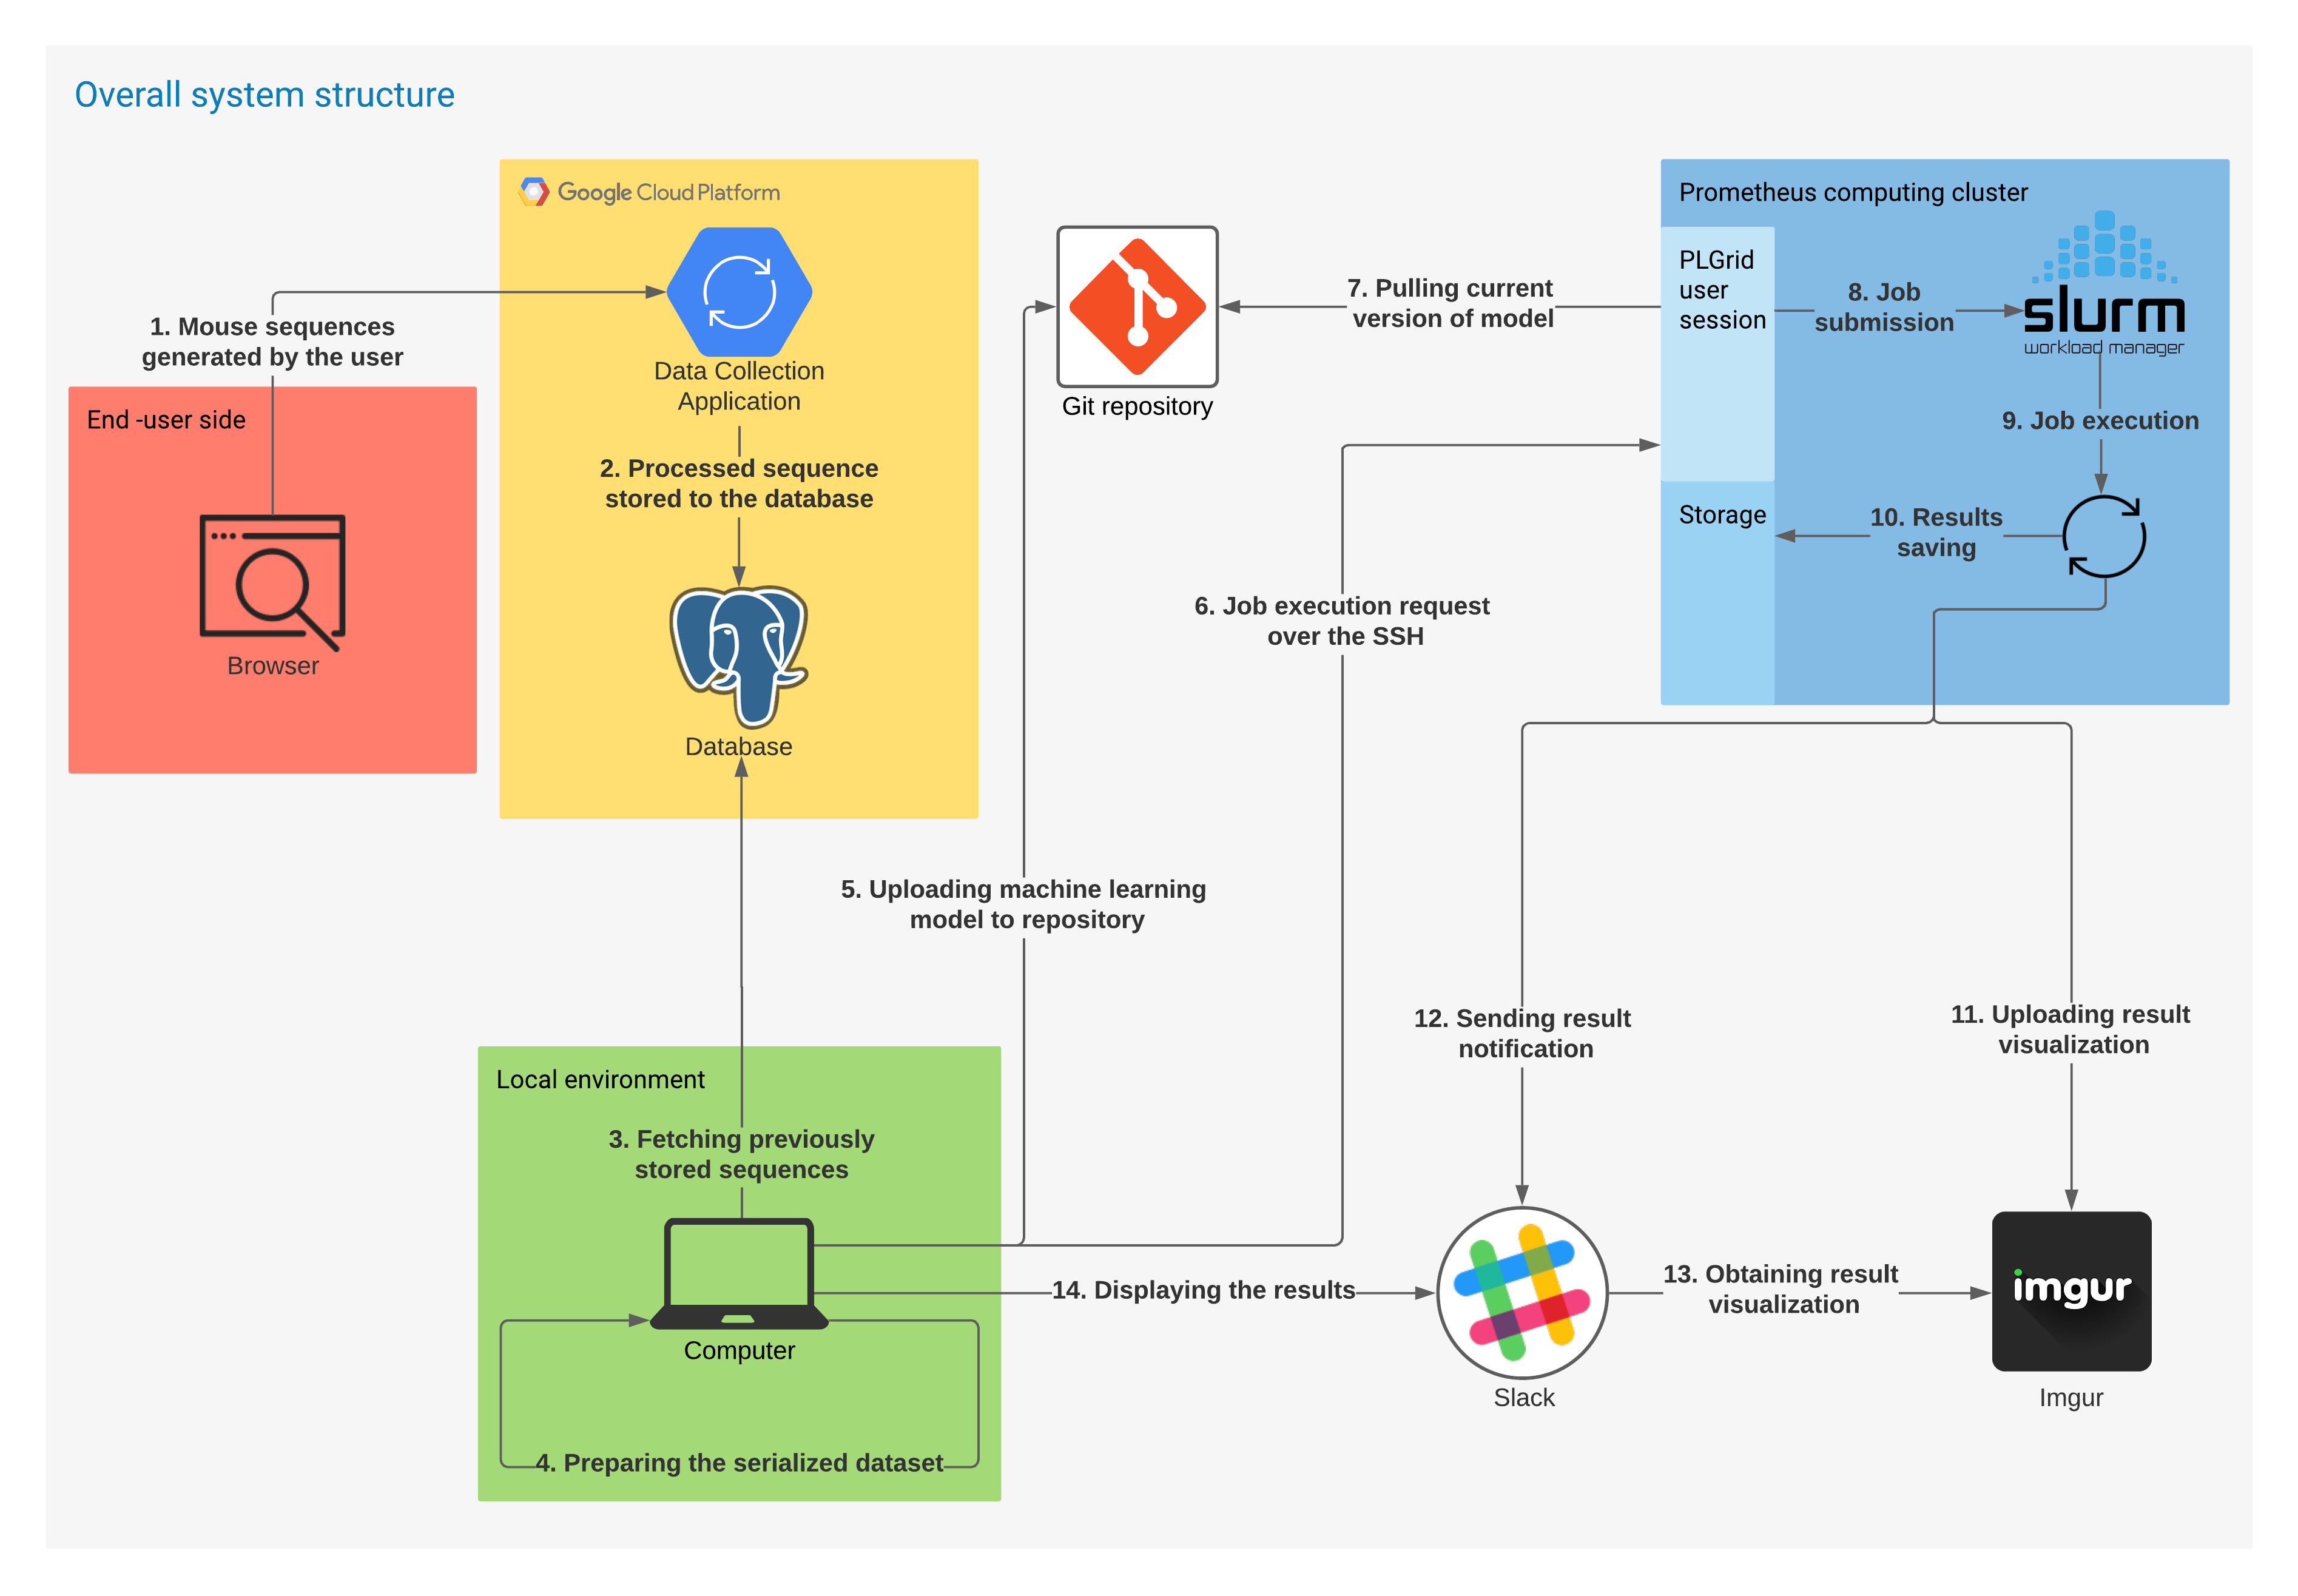
\includegraphics[width=\linewidth]{resources/overall_diagram.png}
    \captionof{figure}{Overall system structure diagram}
    \label{fig:overall_system_structure}
\end{figure}

The entry point for the system is the user's browser that allows the human user as well as a human impersonating bot for access to the prepared website which is hosted on the Internet.
The \mbox{Data Collection}\upperref{itm:data-collection} module which is persisted and operates within a cloud acts as a mouse dynamics data collector, which means that every single mouse event generated by the user on the website is intercepted, transformed and stored in the underlying database (Fig.~\ref{fig:overall_system_structure}, pt. 1 and pt. 2).
The administrator of the presented system is able to retrieve the data from the database in any time (pt. 3).
The downloaded data can be further processed (pt. 4) to the dataset which will be used in machine learning stage.
The administrator of the system should prepare a machine learning model and upload it to the Git repository (pt. 5) which will be then obtained by a computing cluster to perform computation using the model from the observed branch.
Such an approach allows to work on the solution simultaneously by many data scientists and makes it possible to accelerate the research.
The dataset should be uploaded to the computing cluster and persisted in the group's storage that allows using it by many different paralleled computations (not included in the diagram due to decrease of readability).
Each computation is requested from the local computer using prepared Git's `deploy' alias (described in Section~\ref{sec:prometheus-computing-cluster}) that performs a sequence of operations such as establishing the connection to the cluster, fetching the current version of code from the repository and submitting the job to the Slurm\upperref{itm:slurm} workload manager (pt. 6, 7, 8).
The work of the cluster is fully asynchronous because each job is queued and therefore the completion time is unknown.
This is very inconvenient because there is no notification system that allows getting the information about the finished job.
To overcome these limitations, the notification system is proposed as a part of Bot Detection\upperref{itm:bot-detection} module.
The creation of such a system enables the presentation of the results of the computed job in the message as well as the graphs prepared based on the output of the job.
To provide the possibility of sending the images, the notification system uses the external image hosting website called Imgur\upperref{itm:imgur} which allows to upload pictures to the server and host them under the generated \gls{url} (pt. 11).
The results and the graphs are combined into Slack's\upperref{itm:slack} message and then sent to the previously prepared channel by using the webhook \gls{api} (pt. 12, 13).

The further subchapters treat about the implementation details.
At the beginning the Data Collection module is described along with the cloud configuration and performance tests, further, the bot which impersonates the human user and finally the machine learning model alongside the tools such as, among others, a notification module.


\section{Data serialization}\label{sec:data-serialization}
The persisted data from the database were to serve as the input for a machine learning model, however, due to inconvenient usage of SQL queries for such purposes, the serialization tool was developed in order to translate the state of the database records to binary files.
In the presented solution, such files were treated as immutable, so the operation of serialization could have been performed only once, which resulted in the improvement of the required time to read the data by the machine learning model.
Moreover, binary files allowed straightforward sending and storing data in external infrastructures, such as PLGrid\footnote{\url{http://www.plgrid.pl/}}, because it did not require maintenance of database engine in that environment.
Such an approach made it also possible to process data and prepare them in a way that was being required by the machine learning model.

To fulfill these requirements, the serializer and deserializer tools were developed for saving sequences in binary files and further reading those data in Python script.
The serialization was being performed using a tool written in Go\footnote{\url{https://golang.org/}} and provided additional tuning of resulted binary files and configuration of connection to the database.
Among the others the tool allowed to choose the type of event generated by the user such as mouse click or move, minimum sequence length that should have been considered as valid data, minimum screen resolution in order to filter the actions from mobile devices or the time gap between two actions that should have been considered as the boundary between two sequences.
The results of such filtration were being saved in the chosen directory dividing the output into the user's directories and saving each separate sequence in a single file, so the output consisted of many user's directories each containing many single sequence files.
It was possible to use also a so-called one-user mode that enabled generating output data only for a single arbitrary chosen user for debugging purposes.

In order to make serialization uncomplicated and transferable between different programming languages, the serialization framework was used.
At the beginning the chosen one was Apache Avro\footnote{\url{https://avro.apache.org/}} which allows to defining the schema in simple JSON file.
The serialization is performed with help of a library that allows reading schema and saving programming language native objects to binary files.
In the presented solution serialization should have been performed using the library for Go and the deserialization with support of the library for Python, however, they proved to be incompatible which resulted in errors in deserialized data.

To avoid invalid data and to do not spend too much time on finding the bug in those libraries, another approach was taken by applying the Protocol Buffers\footnote{\url{https://developers.google.com/protocol-buffers}} technology.
Protocol Buffers or simply Protobuf is a method of serializing data to the binary form, but the real advantage of it is official multilingual support by generating a serializing code in required programming language.
Protobuf also requires the definition of a schema like Apache Avro, but unlike Avro, the config file format is developed especially for Protobuf, at the same time it is also readable and effortless to write.
Basing on the created schema the code was generated both for Serializer and Deserializer, but in the case of Deserializer, the data was directly read to the Pandas\footnote{\url{https://pandas.pydata.org/}} Dataframe objects, which provided a simple interface to manipulate huge amount of data.

\section{Prometheus computing cluster}\label{sec:prometheus-computing-cluster}
Data processing and machine learning model training and evaluation require a lot of computing resources.
Performing such computations locally, on a single processing core is not the best approach, at least not the most effective method.

To enhance the process of manipulating the collected data, the computing cluster was used as a part of the educational grant issued by the PLGrid.
To make the most out of the computing cluster, plenty of helpers and steering scripts were prepared to automate the process of managing the Prometheus supercomputer.

Prometheus cluster is sharing the resources among multiple users.
Therefore, the computation is scheduled as a job by the SLURM Workload Manager\footnote{SLURM homepage --- \url{https://slurm.schedmd.com/documentation.html}}.
To submit a batch job to the SLURM manager, the input shell script is needed and in this case, the \textit{sbatch\_job\_config} script which contains the job description was prepared.

On the top of the \textit{sbatch} script, a helper shell script exists --- \textit{run-plgrid-job}, which is obtaining useful values that steer the SLURM scheduler as well as triggers the notification job described in previous subsection~\ref{subsec:slack-notifier}.

For automation, the Git version control system was used to implement a very simple continuous delivery system.
The combination of the git versioning system with its aliases allowed to create a \textit{deploy} alias, which was simply performing the pushing to the remote system --- in this case, the Prometheus cluster --- but also connecting to it and submitting the job.
After successfully submitting, the user receives a notification on Slack.
When the job starts, crashes, or finishes properly, the notification is sent again to the Slack.
This gives a very convenient insight into the process and progress of the job without constantly checking for the status manually.
The whole setup can be done easily via the \textit{make} program with prepared \textit{Makefile} file.

\section{Data preprocessing}\label{sec:data-preprocessing}
To fulfill the requirements of the adapted transfer learning model the preprocessing tool was developed alongside a whole bunch of settings.
The collected data sequences are in form of coordinates' series, so it is necessary to represent them as 3-dimensional pictures which are the input to the convolutional neural network.
The described tool allows transferring those sequences into multidimensional arrays of integers and also scale them to the required input size of a used transfer learning model.

\begin{figure}[!hbt]
    \center
    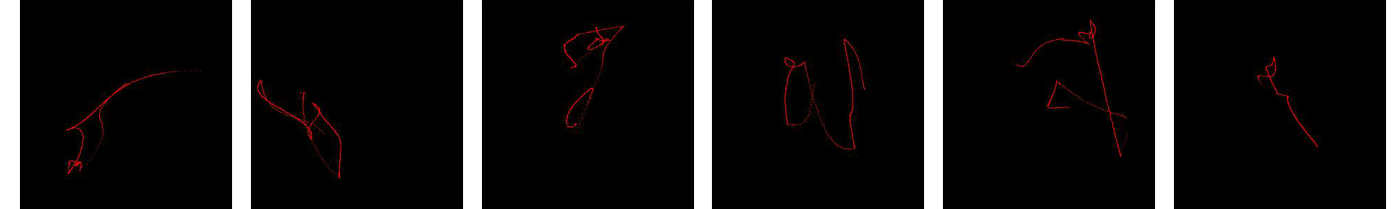
\includegraphics[width=\linewidth]{resources/bot_sequences}
    \captionof{figure}{Collected and preprocessed bot sequences with applied linear interpolation}
    \label{fig:bot_sequences}
\end{figure}
\begin{figure}[!hbt]
    \center
    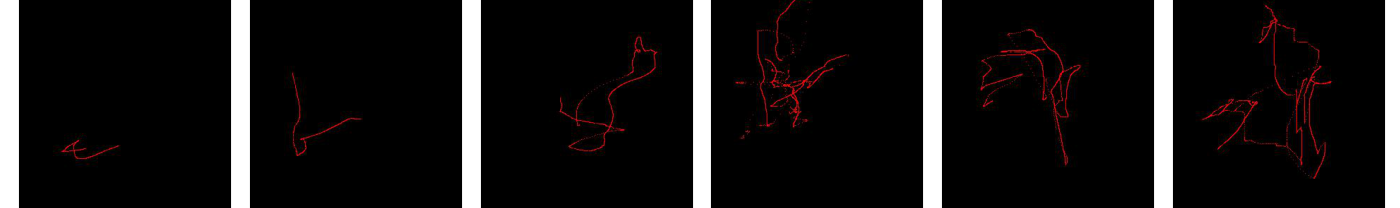
\includegraphics[width=\linewidth]{resources/user_sequences}
    \captionof{figure}{Collected and preprocessed user's sequences with applied linear interpolation}
    \label{fig:user_sequences}
\end{figure}


The data consists of isolated points that are result of discrete sampling, so to improve performance efficiency these points on the "painting" are interpolated using a linear interpolation mechanism.
It was verified on the collected dataset that interpolated data results in better accuracy of a model in comparison to the isolated ones.
The presented tool works also as a splitter between training and testing sets using the provided ratio between them and as a label assigner which allows adding the corresponding labels to the single sequence basing on the provided identifier of the bot user.

Using this tool it is also possible to increase the number of bot samples by using several repetitions of the original bot set in cases of an imbalanced dataset.
The output of the preprocessor is a tuple of training and testing dataset along with labels, which can be directly the input of a neural network model.
\section{Bot Detection module}\label{sec:bot-detection-module}
To validate the consistency and quality of the gathered data the Bot Detection module is introduced.
This module includes various tools and utilities helpful for manipulating the data, model observations and results analysis.
The selected submodules are briefly described in the following paragraphs.
\subsection{CSV writer}\label{subsec:csv-writer}
To persist machine learning model execution results and statistics for later analysis, the outcome data should be stored in a consistent way.
The CSV\footnote{Comma-Separated Values} file is a convenient file format to persist this kind of data because the values from different execution sessions can be easily appended using established schema.
The CSVWriter class introduces methods for appending the data to the file. The other helper methods allow for checking the correctness of the file and its content.

\paragraph{Uploading charts on web}\label{para:charts-web-uploading}
To see whether the machine learning model is actually getting better during the training process, accuracy and loss charts can be used as a really helpful method to determine the learning curve.
To receive a `live' preview of the model execution results with charts as a notification in Slack communicator, the charts needed to be stored somewhere on the internet.
The easiest way to achieve this requirement was to use the \gls{api} of the Imgur\upperref{itm:imgur} platform.
Thanks to the official module that can be used with Python, the platform offers a simple way to upload the images to the service and returns the \gls{url} to the stored image when successfully uploaded.

\subsection{Results terminating}\label{subsec:results-terminating}
When the model was executing the calculations multiple times, the results for each iteration were collected.
This is giving a really interesting insight into the model and its stability.
The tool called \mbox{\textit{ResultTerminator}} was serving this purpose.
The helper methods were used to determine whether the file is existing already and if not creating it.
To avoid concurrent saving problems, the file is achieving the lock and releasing it when the content is successfully saved to CSV file.

\subsection{Slack notifier}\label{subsec:slack-notifier}
Working with PLGrid infrastructure and running a job on the Prometheus computing cluster was very helpful in terms of delegating the great amount of computing load onto external resources.
However, this solution has its downsides.
One of the major issues is the job queueing mechanism, which does not determine when the job will be executed and therefore it requires constant manual checking for results.
To avoid that somehow, the authors prepared a custom mechanism, that can monitor the status of the job and notify the Prometheus user through the Slack\footnote{\url{https://slack.com/} – a messaging app for teams} channel.
Three following message templates were prepared for the purpose of notification:
\begin{enumerate}
    \item Simple message --- Generic message type build as a \gls{json} template with help of Builder design pattern to have flexibility in customizing the message.
    \item Pending job message --- able to notify about: job title, reporter, commit hash, job registration date and time, header for app preview, info message taken from a commit.
    Build as a special case of Simple type message.
    \item Results message --- The most complex message with all the statistic results produced as a result of the model computation.
    Prepared as a \gls{json} template with the help of the Builder design pattern.
\end{enumerate}

To avoid that somehow, the authors prepared a custom mechanism, that can monitor the status of the job and notify the Prometheus user through the Slack channel using observability-like architecture.

% How to ref to paragraph: https://tex.stackexchange.com/a/334756
\paragraph{Statistics calculation}\label{para:statistics-calculation}
The prepared model was intended to be running several times in order to measure the consistency and stability of the results.
To properly measure and visualize the model scores, a dedicated module for processing the results was prepared.
Two main core parts can be distinguished --- the plotting utilities and the statistics metrics calculation submodule.

The submodule for calculating metrics allows for producing the mean value of accuracy, model loss, percentage of \gls{far} and \gls{frr}, number of true negatives, true positives, false negatives and false positives.
The plotting submodule allows for producing the following charts:
\begin{samepage}
    \begin{itemize}
        \item[---] generic linear plot creation used to display accuracy and loss charts,
        \item[---] creating the accuracy percentile histogram.
    \end{itemize}
\end{samepage}

The above metrics and functionalities are designed to produce the averaged model results for multiple executions.
The developed model is stable and the error is irrelevant between each execution.

\section{Machine learning model}\label{sec:machine-learning-model}
The machine learning model prepared and trained on the collected dataset was the part of the data evaluation final part.
Google Cloud Services are able to handle the deployment of the whole system efficiently.
However, this form of hosting and maintaining the infrastructure of the application comes with its price.
The whole infrastructure was running for about two months and during this time generated the cost of a total \$300.
This amount of cash is the highest financial outlay that could have been incurred by the authors of the work since no other scholarship than PLGrid computation cluster was granted for the purpose of preparing the thesis.
Longer exposure on the Web would cost extra money, that could not be afforded.
The other matter is that the engineering thesis defending has its deadline specified, thus the project has been carefully thought-out in the manner of time since the beginning of the implementation.
In order to meet the adopted milestones and goals, the data collection period had to follow strict deadlines.
The duration of the period when the data was collected could not be extended to broader terms, which resulted in relatively small dataset.

The first remedy for a small amount of collected data was to use the transfer learning technique.
The base feature vector for transferring to the bot recognition domain was taken from the TensorFlow Hub\upperref{itm:tensorflow-hub} website.
The model was pre-trained on ImageNet dataset\upperref{itm:image-net} using the architecture of Inception V3, which is showing a great potential in the terms of the computer vision with improved performance over the previous versions, with a relatively modest computation cost~\cite{inception-v3}.
The model was built with the following dimensions of $299$\texttimes$299$\texttimes$3$ for the data input.
The topmost layers were added for the transferring and tuning to the bot detection domain.

The first attempts were not very exciting because of the limited amount of samples.
The model behaved unilaterally which means that the dominance of user's samples outshone the bot samples.
The different approaches were taken to improve the performance such as linear interpolation by connecting the points in recorded sequences.
Each used sequence originally consisted of many single discrete points without any additional pieces of information.
Interpolation provided an order between discrete coordinates and allowed feeding the neural network with additional information.

Another considered approach was a manipulation of the input data size.
The user's sequences were limited to the number of total bot sequences.
This solution was aimed to balance the dataset at the cost of fewer data.
The results of this approach turned out to be insufficient --- because of the total amount of bot sequences, the total size of the dataset drastically shrank, which resulted in a performance deterioration.
On the other hand, the duplication of the bot sequences was used.
The idea was similar to the one discussed before, but instead of reducing, the number of bot samples was increased by using a single sample several times.
It resulted in an artificially balanced dataset.
However, this approach did not increase performance at all.

Manipulation of the distribution of labels between training and testing dataset was also considered.
It was done by performing either an equalization of the total number of both types in the testing dataset and the distribution of samples between both datasets.
The first solution did not affect model performance, but the second one slightly improved overall performance if the ratio was close to 50:50.
When the number of training samples was significantly greater than testing ones, the accuracy decreased due to a very small number of bot samples in testing dataset.

Yet another attempt to reduce the impact of the small dataset was changing the dataset itself.
The developed serializing tool made it possible to create a few datasets from recorded data with different minimal sequence length limits.
Using longer sequences meant that the overall number of them would be smaller.
The authors tested several ones and found out that the best performance was for a length equal to 50.

To overcome the described issue, another technique called data augmentation was used.
As stated in the "The Effectiveness of Data Augmentation in Image Classification using Deep Learning" by Perez et al. article --- "It is common knowledge that the more data an \gls{ml} algorithm has access to, the more effective it can be.
Even when the data is of lower quality, algorithms can actually perform better, as long as useful data can be extracted by the model from the original data set"~\cite{augmentation}.
The main idea of this approach is to increase the samples of the dataset by using the same sample several times, but each time slightly transforming it.
The transformation is based on operations such as rotations, zooming, and flipping the original sample with some probability to do so, so each artificially generated sample should be slightly different than the others.
This approach allows significantly increasing the size of the dataset.
In the presented solution, it was done by development of augmentation script using Augmentor\upperref{itm:augmentor} package for Python.
Each of the datasets (users and bot) was extended to 30,000 samples which results in a total of 60,000 samples from just 639 original samples.
The ratio between the training and testing part was set to 80:20, so the network used for the training 48,000 samples and for the testing 12,000.
For the optimization of the model, the optimizer called Adam was used along with the learning rate exponential decay set initially to $10^{-4}$.
The decay rate was equal to 0.96 and the decay steps were set to $10^{5}$.
The loss function was set to the binary cross entropy loss due to the binary classification problem.

To save time and optimize resources usage, the first approach for running the model was to execute it in a multi-threaded way.
For this purpose, the module which was facilitating that was created.
Soon this approach was abandoned due to the encountered problems.
The main problem was that the SLURM manager is not able to split the resources in a way to the multithreaded approach to be sensible.
The resources were assigned to the whole computing node on which only 2 \gls{gpu} cards were able to be allocated.
This caused the problem of many machine learning models trying to run on a single card.

When run on the Prometheus cluster, the better approach was to split the computation between two \gls{gpu}s and run the model sequentially.
For this purpose, the Mirrored Strategy distribution technique from the TensorFlow library was used whereas training is split across multiple replicas.
Thanks to the split and the computing power of \gls{gpu}, single execution is faster, thus can be multiplied several times.

\subsection{Model execution strategy}\label{subsec:model-execution-strategy}
As stated before, the model is running several times.
To save time and optimize resources usage, the first approach for running the model was to execute it in a multi-threaded way.
For this purpose, the module which was facilitating that was created.
Soon this approach was abandoned due to the encountered problems.

When run on the Prometheus cluster, the better approach was to split the computation between two GPUs and run the model sequentially.
For this purpose, the Mirrored Strategy distribution technique from the TensorFlow library was used whereas training is split across multiple replicas.
Thanks to the split and the computing power of GPU, single execution is fast, thus can be multiplied several times.

\chapter{Final results and summary discussion}\label{ch:final-results-and-summary-discussion}


\section{Results}\label{sec:results}

Presented model was trained and tested using various parameters.
The changes were affected by the input data as well as the neural network parameters.
The final dataset properties used to train the presented model are described in \mbox{Tab.~\ref{tab:dataset}}.
The input picture size was forced by a used transfer learning model.
This limitation had an effect on resizing original pictures of sequences to the required one by the used neural network.

\begin{table}[!hbt]
    \centering
    \begin{minipage}{.49\textwidth}
        \centering
        \captionsetup{width=\linewidth}
        \captionof{table}{Dataset properties} \label{tab:dataset}
        \begin{tabular}{p{0.6\textwidth}p{0.29\textwidth}}
            \hline
            Users                    & 46                 \\ \hline
            Human users              & 45                 \\ \hline
            Bot users                & 1                  \\ \hline
            Sequences                & 639                \\ \hline
            Minimal sequence length  & 50                 \\ \hline
            Model input picture size & 299 x 299 {[}px{]} \\ \hline
        \end{tabular}
    \end{minipage}
    \hfill
    \begin{minipage}{.5\textwidth}
        \centering
        \captionsetup{width=\linewidth}
        \captionof{table}{Confusion matrix values} \label{tab:confusion-matrix}
        \begin{tabular}{p{0.50\textwidth}p{0.12\textwidth}}
            \hline
            False negatives       & 19    \\ \hline
            False positives       & 0     \\ \hline
            True negatives        & 327   \\ \hline
            True positives        & 0     \\ \hline
            False rejection rate  & 100\% \\ \hline
            False acceptance rate & 0\%   \\ \hline
        \end{tabular}
    \end{minipage}
\end{table}

The total amount of sequences depends on the minimal sequence length, because sequences that were shorter than \num{50} were simply rejected.
The sequence split point was established by the time interval between two consecutive actions and in presented work was fixed to \num{1} second.
The minimal sequence length was fixed based on several attempts.
Shorter sequences than the determined ones resulted in apparently lower accuracy, when longer did not improve performance at all.
The length of \num{50} seemed to be the golden mean between accuracy and amount of sequences.

The charts presented on the \mbox{Fig.~\ref{fig:accuracy} and Fig.~\ref{fig:loss}} show that model accuracy reaches the level of \num{94}\% with \num{69.5}\% value of loss function.
It can be seen that model accuracy during the testing part is in most epochs higher than the one in the training.
It is caused by an imbalanced dataset which was the input for the presented model, where
the amount of user data for testing was greater than the bot one.
It is direct effect of having more user data in the whole dataset.
The impact is also seen on the loss function chart \mbox{(Fig.~\ref{fig:loss})} where values are lower in the testing part.

\begin{figure}[!hbt]
    \centering
    \begin{minipage}{.5\textwidth}
        \centering
        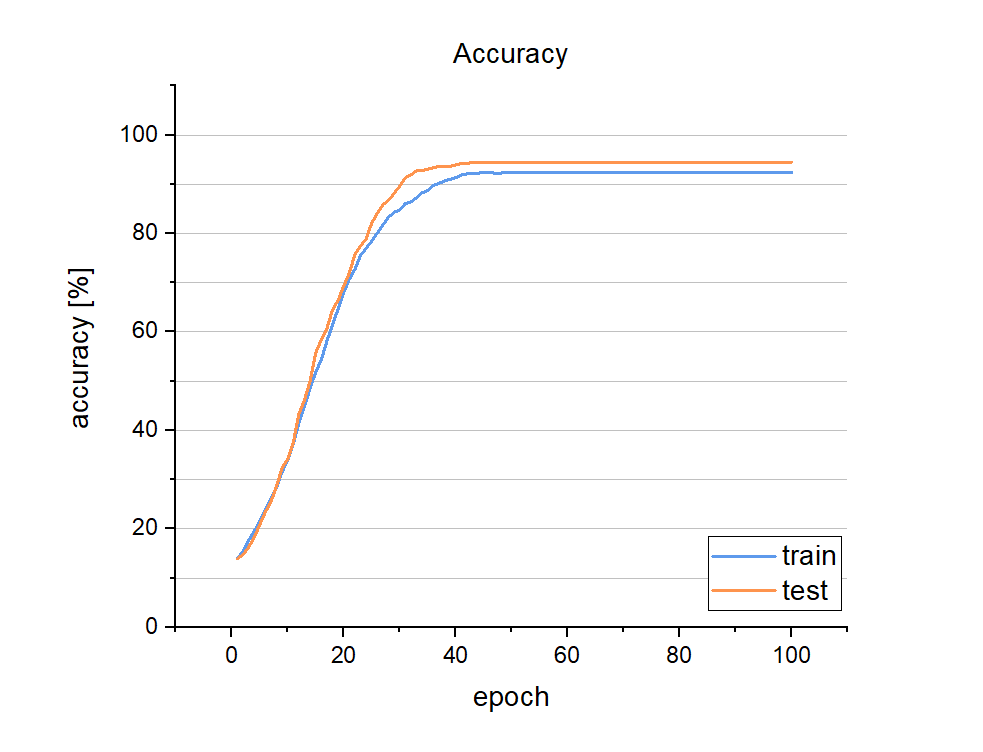
\includegraphics[width=\linewidth]{resources/accuracy.png}
        \captionsetup{width=\linewidth}
        \captionof{figure}{Accuracy of presented model}
        \label{fig:accuracy}
    \end{minipage}%
    \begin{minipage}{.5\textwidth}
        \centering
        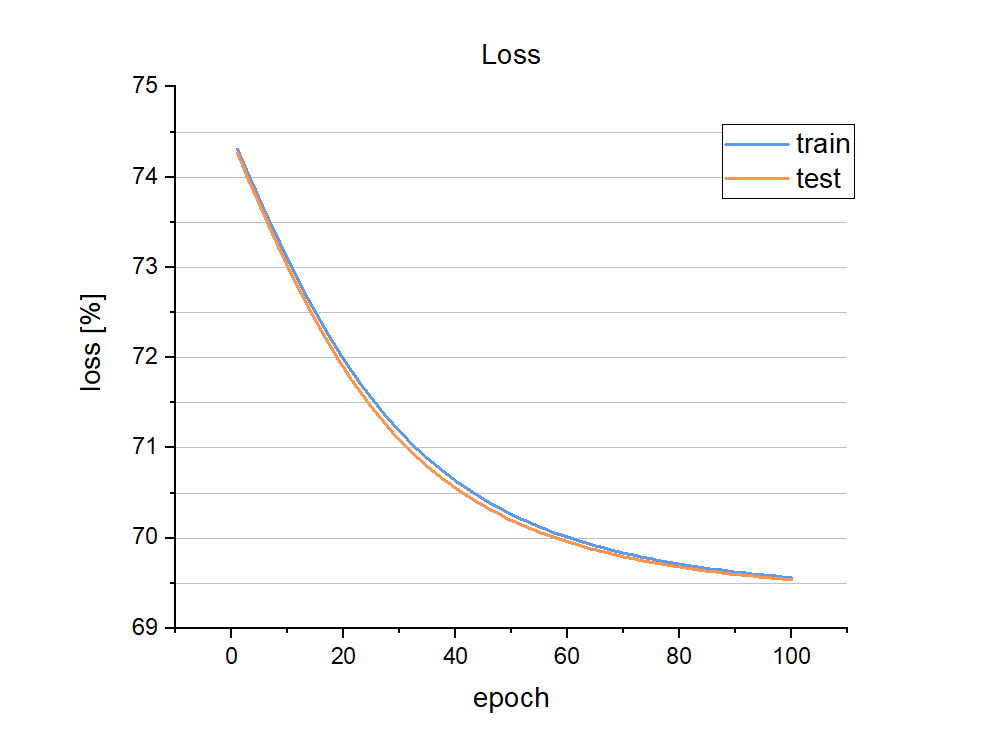
\includegraphics[width=\linewidth]{resources/loss.png}
        \captionsetup{width=\linewidth}
        \captionof{figure}{Value of loss function used in model}
        \label{fig:loss}
    \end{minipage}
\end{figure}

Moreover, due to that inappropriate data, model had some problems with prediction.
At the beginning of the learning procedure, user and bot data were treated with equal importance.
With the successive epochs, user data outshone bot dataset.
It can be seen \mbox{(Tab.~\ref{tab:confusion-matrix})} that after the learning process, there were no true positives, which suggests that the model learned only one type of data.
The model always predicted that the input data was the user's one.
It is the result of a large amount of user data in comparison to bot sequences, whereas it is not the result of having only one bot user and many human users, because each user's sequence was joined into a global one.

Chong et al.~\cite{Main} present similar approach to related problem, but the results achieved in this study show that the presented solution behaves unilaterally.
In many cases from cited work, authors achieved very low values of FRR\footnote{False Rejection Rate} and FAR\footnote{False Acceptance Rate}\@.
In this work, using CNN's\footnote{Convolutional Neural Network} as a core of a solution, totally different results were achieved.
The authors of this study consider the imbalanced dataset as the main foundation of that unexpected behavior.
Despite the numerous efforts taken, the results are unsatisfactory.
The obtained accuracy chart (Fig.~\ref{fig:accuracy}) is somehow expected due to the dominance of one kind of data in the binary selection problem.
However, the loss function (Fig.~\ref{fig:loss}) as well as confusion matrix (Tab.~\ref{tab:confusion-matrix}) have undesirable values.


\section{Limitations, conditions and problems}\label{sec:limitations-conditions-problems}
Although the model was considered using different sets of parameters and various approaches, it did not perform well.
Due to certain limitations, some aspects of the model performance could not have been improved.
Some problems that have a great impact on the overall results are described in the following sections.

\subsection{Dataset limitation}\label{subsec:dataset-limitation}
The main reason for poor performance has to be an insufficient dataset used in the study.
The search for proper and publicly available data resulted in failure.
In other related works, like Chong et al.~\cite{Main} or Antal et al.~\cite{balabit1} points at the Balabit Mouse Challenge Dataset\footnote{\url{https://github.com/balabit/Mouse-Dynamics-Challenge}} as the most popular and comprehensive, yet still quite small data source for mouse sequences and behaviors.
However, this dataset is not appropriate for the problem considered in this study.

The Balabit dataset consists of user sessions recorded on the remote machine.
The data includes the timing and position of the mouse cursor of ten different users.
The split dataset represents training sessions and test sessions.

In the training sessions, one can find \num{65} legitimate sessions of various lengths, wherein total gives \num{2253871} rows of registered user mouse actions.\\
Test sessions consist of \num{1611} shorter sequences, that in total have \num{2357714} recorded actions, where during the session execution of the legal user, the illegitimate action happens --- the session is taken over by another user.
Illegal sessions are the mix of two legitimate users, and when the model considers the example it should assume one user, that is then interrupted and replaced by another user somewhere between the session.

This data does not relate to the problem given in the scope of this work --- the model that can distinguish legitimate human user and non-human bot behavior is taken into consideration.
This particular case is derived from the general problem of distinguishing two or more users and represents a more specific case of using mouse behavioral biometrics.

\subsection{Custom dataset research participation limitation}\label{subsec:custom-dataset-research}
Since no public dataset is available, there was an attempt to collect exclusive and dedicated data for purpose of the study.
The custom environment\footnote{\url{https://github.com/Mouse-BB-Team/Data-Collection}} created as a playground for research participants was designed to collect and record the mouse data, but it did not serve the responsiveness of a real commercial website, and therefore it may be causing some confusion among the subject users.
By that means, data collecting was in some kind suggestive and task-oriented.
Given factors could have a negative impact on the quality of the collected data.

The other thing is that participation in the study was completely voluntary and community-based.
The advertisement for the ongoing study was posted on a couple of Facebook\footnote{https://facebook.com/} groups, which was the most available and large user community base.
However, such an approach resulted in non-supervised data gathering, and therefore some user actions could not be assessed as properly executed and caused disturbances and noises in the set.

The research gathered \num{63} unique users.
Overall user mouse actions collected are equal to \num{334184} rows.
The number of bot actions registered and collected is equal to only \num{24791} rows.\\
Such an uneven ratio of the data made the dataset imbalanced, which resulted in the model making assumptions about every sequence biased towards the class of human users.
Training set contained about \num{269231} bot and user sequences, whereas the test set contained \num{89744} sequences --- even using transfer learning technique, the dataset was too small for efficient model training.

\subsection{Finance limitation}\label{subsec:finance-limitation}
Another problem encountered when preparing the thesis was the limit of the finance intended.\\
Because the research was planned to reach many different users it had to be deployed and hosted on trusted and reliable resources.

Cloud services are really convenient way to handle such a project --- the hosting, computation, and storage resources can be acquired on-demand, with no time and commitment.
In the variety of different cloud solutions, in this case, the Google Cloud Platform\footnote{\url{https://cloud.google.com/}} was selected and used.

Google cloud services are able to handle the deployment of the whole system efficiently.
This form of hosting and maintaining the infrastructure of the application comes with its price.
The whole infrastructure was running for about two months and during this time generated the cost of total \$\num{300}.
This amount of cash is the highest financial outlay that could have been incurred by the authors of the work, since no other scholarship than PLGrid\footnote{\url{http://www.plgrid.pl/}} computation cluster was granted for the purpose of preparing the thesis.
Longer exposure on the web would cost extra money, that could not be afforded.

\subsection{Time limitation}\label{subsec:time-limitation}
Engineering thesis defending has its term specified, thus the project has been carefully thought-out in the manner of time since the beginning of the implementation.
In order to meet the adopted milestones and goals, the data collection period had to follow strict deadlines.
The duration of the period when the data was collected could not be extended to broader terms, thus the research and the voluntary participation in data collection were canceled during the further implementation of the project --- the bot detection part\footnote{\url{https://github.com/Mouse-BB-Team/Bot-Detection}}, where the machine learning model was in build.

\section{Conclusions and further study}\label{sec:conclusions-and-further-study}

\subsection{Summary}\label{subsec:summary}
During the work on the presented solution, the steps to limit the impact of the imbalanced dataset were taken.
As an example, linear interpolation was used by connecting the points in recorded sequences.
Each used sequence originally consisted of many single discrete points without any additional pieces of information.
Interpolation provided an order between discrete coordinates and allowed feeding the neural network with additional information.

Another considered approach was a manipulation of the input data size.
The user's sequences were limited to the number of total bot sequences.
This solution was aimed to balance the dataset at the cost of fewer data.
The results of this approach turned out insufficient.
Because of the total amount of bot sequences, the total size of the dataset drastically shrank, which resulted in a performance deterioration.
On the other hand, the duplication of the bot sequences was used.
The idea was similar to the one before, but instead of reducing, the number of bot samples was increased by using a single sample several times.
It resulted in an artificially balanced dataset.
However, this approach did not increase performance at all.

Manipulation of the distribution of labels between training and testing dataset was also considered.
It was done by performing either an equalization of the total number of both types in the testing dataset and the distribution of samples between both datasets.
The first solution did not affect model performance, but the second one slightly improved overall performance if the ratio was close to \num{50}:\num{50}.
When the number of training samples was significantly greater than testing ones, the accuracy decreased due to a very small number of bot samples in testing dataset.

Yet another attempt to reduce the impact of the inappropriate dataset was changing the dataset itself.
The developed serializing tool made it possible to create a few datasets from recorded data with different minimal sequence length limits.
Using longer sequences meant that the overall number of them would be smaller.
The authors tested several ones and found out that the best performance was for a length equal to \num{50}, as it was mentioned before.

All of the presented approaches tended to minimize the dataset problem.
Some of them slightly improved performance and those were considered in the final solution.
Despite the efforts and attempts for improving the model, the described problem significantly worsened the performance of the model.

\subsection{Further study}\label{subsec:further-study}
According to the described issues, the authors find further study mainly in the improvement of the dataset.
Some efforts may be taken to extend the size of the recorded data.
Firstly, recording sequences of a bigger group of users may be proposed as a solution, especially enlarge the bot users to prevent imbalance.
Such a solution should improve the overall performance of the model or at least suggest other problems related to the quality of the dataset.\\
If the quality of the recorded samples would be inappropriate, the collection module\footnote{\url{https://github.com/Mouse-BB-Team/Data-Collection}} should be reviewed and improved.
The main object of interest should be the method of gathering the samples.
Delays and synchronization that can disturb the reliability of the data may be considered as a major area of study.

The different approach that may be taken into consideration is another machine learning model.
In the presented solution, the focus was on the two-dimensional convolutional neural network, taking an example from related works like Chong et al.~\cite{Main} and Wei et al.~\cite{Inspiration}.
The work~\cite{Main} also shows other solutions, especially recursive neural networks.
Those kinds of neural networks are very popular in problems where the order and time intervals between samples have natural interpretations.
The problem which is described in this work also has similar properties.

These two described areas of study are found by the authors as the major to improve performance and reliability.
To deliver a safe and reliable solution to the commercial market further study is necessary.


% itd.
% \appendix
% \include{dodatekA}
% \include{dodatekB}
% itd.

\printbibliography

\end{document}
